% Outils Latex

%************************************************************************
%									BASE
%************************************************************************

\documentclass[a4paper,oneside]{article}
%Compilé avec MacTex

%Langage
\usepackage[french]{babel} 
\usepackage[utf8]{inputenc}
\usepackage{hyperref} % références dans pdf
\usepackage{lmodern}

%Géométrie
\setlength{\parindent}{17pt}%Pour les indentations au début de paragraphe
\setlength{\parskip}{7pt}%Pour espaces entre paragraphes
\usepackage{rotating} % pour rotatebox
\usepackage{geometry}
\geometry{hmargin=2.5cm,vmargin=3.5cm}
\usepackage{pifont}%liste à puce


%Images
\usepackage{graphicx} % pour images
\usepackage[tt]{titlepic}%mettre une image sur une page de titre
\usepackage{caption}
\usepackage{epstopdf}
\usepackage{gnuplottex}% pour faire du gnuplot directement dans le latex


%Maths & Symboles
\usepackage{amsmath}
\usepackage{amssymb}
\usepackage{mathrsfs}
\usepackage{mathenv}
\usepackage{sistyle}
\usepackage{ulem} %pour souligner 2 fois
\usepackage{flexisym}
%\usepackage{SIunitx}
%\usepackage{siunitx}%pour les unités SI

%Puces des items
\usepackage{enumitem}
\usepackage{xcolor}

%Code
%\usepackage{listings}


%En tête, Annexes, Bibliographie
\usepackage{appendix} % pour les annexes
\pagestyle{headings} % pour en têtes
\usepackage[nottoc, notlof, notlot]{tocbibind} % pour que bibliographie soit comprise comme un chapitre ou section
\usepackage{chngpage}
%\usepackage{fancyhdr} %pour faire une entête personnalisée
%\pagestyle{fancy}%pour faire une entête personnalisée
%\usepackage{lastpage}

%En tête perso
\renewcommand{\headrulewidth}{0.5pt}
\fancyhead[L]{Quentin Berg\'e\\ Valentin Lamberet}
\fancyhead[R]{Milieux Poreux}
%Pied de page perso
%\renewcommand{\footrulewidth}{1pt}
%\fancyfoot[C]{\textbf{page \thepage}} 
%\fancyfoot[L]{truc}
%\fancyfoot[R]{\leftmark}

%Déclarations
\DeclareTextSymbol{\degre}{OT1}{23} %pour le symbole degré


%Bigcenter pour images
\makeatletter % pour /bigcenter qui permet de s'affranchir des marges pour les images
\newskip\@bigflushglue \@bigflushglue = -100pt plus 1fil
\def\bigcenter{\trivlist \bigcentering\item\relax}
\def\bigcentering{\let\\\@centercr\rightskip\@bigflushglue%
\leftskip\@bigflushglue
\parindent\z@\parfillskip\z@skip}
\def\endbigcenter{\endtrivlist}
\makeatother




\begin{document}

%Pour Code
\lstset{language=Matlab,breaklines=true,keepspaces=true,                 % how far the line-numbers are from the code
  %numberstyle=\normal,numbers=left,                    % where to put the line-numbers; possible values are (none, left, right)
  %numbersep=5pt,   % the style that is used for the line-numbers
  frame=single, xleftmargin=2em}
\lstset{literate=
  {á}{{\'a}}1 {é}{{\'e}}1 {í}{{\'i}}1 {ó}{{\'o}}1 {ú}{{\'u}}1
  {Á}{{\'A}}1 {É}{{\'E}}1 {Í}{{\'I}}1 {Ó}{{\'O}}1 {Ú}{{\'U}}1
  {à}{{\`a}}1 {è}{{\`e}}1 {ì}{{\`i}}1 {ò}{{\`o}}1 {ù}{{\`u}}1
  {À}{{\`A}}1 {È}{{\'E}}1 {Ì}{{\`I}}1 {Ò}{{\`O}}1 {Ù}{{\`U}}1
  {ä}{{\"a}}1 {ë}{{\"e}}1 {ï}{{\"i}}1 {ö}{{\"o}}1 {ü}{{\"u}}1
  {Ä}{{\"A}}1 {Ë}{{\"E}}1 {Ï}{{\"I}}1 {Ö}{{\"O}}1 {Ü}{{\"U}}1
  {â}{{\^a}}1 {ê}{{\^e}}1 {î}{{\^i}}1 {ô}{{\^o}}1 {û}{{\^u}}1
  {Â}{{\^A}}1 {Ê}{{\^E}}1 {Î}{{\^I}}1 {Ô}{{\^O}}1 {Û}{{\^U}}1
  {Ã}{{\~A}}1 {ã}{{\~a}}1 {Õ}{{\~O}}1 {õ}{{\~o}}1
  {œ}{{\oe}}1 {Œ}{{\OE}}1 {æ}{{\ae}}1 {Æ}{{\AE}}1 {ß}{{\ss}}1
  {ű}{{\H{u}}}1 {Ű}{{\H{U}}}1 {ő}{{\H{o}}}1 {Ő}{{\H{O}}}1
  {ç}{{\c c}}1 {Ç}{{\c C}}1 {ø}{{\o}}1 {å}{{\r a}}1 {Å}{{\r A}}1
  {€}{{\euro}}1 {£}{{\pounds}}1 {«}{{\guillemotleft}}1
  {»}{{\guillemotright}}1 {ñ}{{\~n}}1 {Ñ}{{\~N}}1 {¿}{{?`}}1
}




%% Definitions du chapitre pour simplifier la frappe
\def\ua{\underline a}
\def\un{\underline n}
\def\uQ{\underline Q}
\def\cD{{\cal D}}
\def\cF{{\cal F}}
\def\cV{{\cal V}}
\def\dcD{\partial{\cal D}}
\def\cC{{\cal C}}
\def\dOmega{\partial{\Omega}}
\def\inttt{\int\!\!\int\!\!\int}
\def\dsdt{\frac{d}{d t}}
\def\pdsdt{\frac{\partial}{\partial t}}
\def\pdsdtc{\frac{\partial c}{\partial t}}
\def\hmic{h_{\rm mic}}
\def\hmac{h_{\rm mac}}
\def\cFsurf{{\cal F}_{\rm surf}}
\def\cFvol{{\cal F}_{\rm vol}}
\def\div{{\rm div\,}}
\def\ugrad{\underline{\rm grad}\,}
\def\eint{e_{\rm int}}
\def\cEint{{\cal E}_{\rm int}}
\def\iiint{{\int\!\!\!\int\!\!\!\int}}
\def\iint{{\int\!\!\!\int}}
%************************************************************************
%									GROS TITRE
%************************************************************************


\begin{titlepage} % Suppresses headers and footers on the title page

	\centering % Centre everything on the title page

	\scshape % Use small caps for all text on the title page

	\vspace*{\baselineskip} % White space at the top of the page


	\rule{\textwidth}{1.6pt}\vspace*{-\baselineskip}\vspace*{2pt}
	 % Thick horizontal rule
	\rule{\textwidth}{0.4pt} % Thin horizontal rule

	\vspace{0.75\baselineskip} % Whitespace above the title

	{\LARGE Bureau d'\'Etudes :\\
	\vspace{0.75\baselineskip}
	Alimentation en Eau Potable du village d'Uzemain \\
	} % Title

	\vspace{1\baselineskip} % Whitespace below the title
	\rule{\textwidth}{0.4pt}\vspace*{-\baselineskip}\vspace*{3.2pt}
	 % Thin horizontal rule
	\rule{\textwidth}{1.6pt} % Thick horizontal rule
	\vspace{2\baselineskip} % Whitespace after the title block

	%------------------------------------------------
	%	Subtitle
	%------------------------------------------------

	% Subtitle or further description
	Hydraulique en Charge

	\vspace*{3\baselineskip} % Whitespace under the subtitle

	%------------------------------------------------
	%	Editor(s)
	%------------------------------------------------


	\vspace{0.5\baselineskip} % Whitespace before the editors

	{\scshape\Large Quentin Bergé \\} % Editor list

	\vspace{0.5\baselineskip} % Whitespace below the editor list

	\textit{ENSEEIHT} % Editor affiliation

	\vfill % Whitespace between editor names and publisher logo

	%------------------------------------------------
	%	Publisher
	%------------------------------------------------

	
\includegraphics[scale=0.8]{logoN7.png} % changer logo

	\vspace{0.3\baselineskip} % Whitespace under the publisher logo

Juin 2019 % Publication year
\end{titlepage}
\newpage

%Table des Matières
\tableofcontents
\newpage

\end{document}

%************************************************************************
%									PETIT TITRE
%************************************************************************

\begin{center}
\rule{8cm}{0.5pt}\\% % Thin horizontal rule
	%\vspace{0.2\baselineskip} % Whitespace above the title
\Large{TD1 Apprentis 2019}\\
\rule{8cm}{0.5pt}%
\end{center}

%************************************************************************
%							Juxtaposer 2 images
%************************************************************************

\begin{figure}[h]
    \begin{minipage}[c]{.46\linewidth}
        \centering
        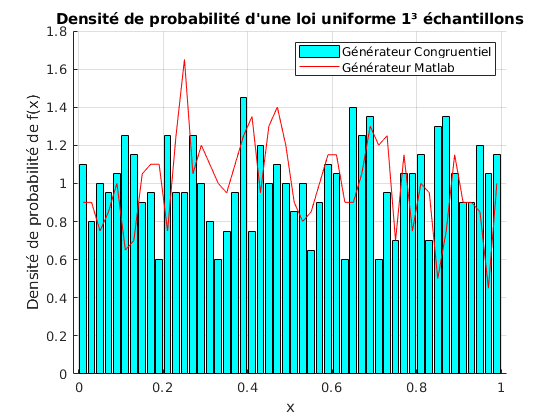
\includegraphics[scale=0.5]{../Exercice1/N=1000.png}
        \caption{$10^3$ échantillons}
    \end{minipage}
    \hfill%
    \begin{minipage}[c]{.46\linewidth}
        \centering
        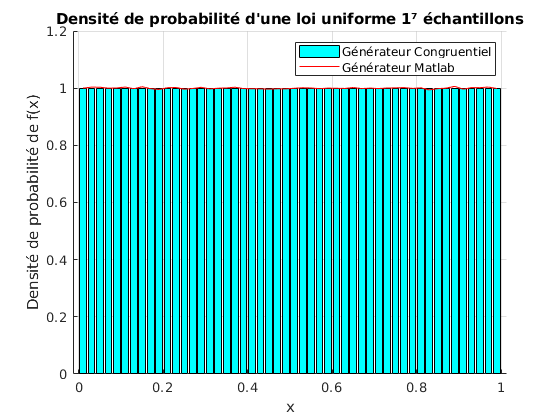
\includegraphics[scale=0.5]{../Exercice1/N=10000000.png}
        \caption{$10^7$ échantillons}
    \end{minipage}
\end{figure}

%************************************************************************
%							Images Pas dans même dossier
%************************************************************************

\begin{figure}[h!]
\bigcenter
\includegraphics[scale=0.8]{../Permanent/Vitesseinf.PNG}
\caption{Tuyaux dont les vitesses sont supérieures à 0,1 $m/s$}
\end{figure}

%************************************************************************
%							Mettre une figure de cote
%************************************************************************
\begin{sidewaysfigure}
\centering
\includegraphics[scale=0.6]{gantlaser.JPG}
\caption{Diagramme de Gantt}
\end{sidewaysfigure}

%************************************************************************
%							Tableau Légendé
%************************************************************************

\begin{center}
\begin{tabular}{|c|c|c|}

 \hline
 Solution 1 & Solution 2 & Solution 3\\
 \hline
 1207.2 & 1421.48 & 1107.5 \\

 \hline
\end{tabular}
\captionof{table}{Coût de fonctionnement journalier des différentes solutions (en euros)}
 \end{center}

 %************************************************************************
 %							Pas d'Alinéa
 %************************************************************************

\noindent

 %************************************************************************
 %							 Texte Brut
 %************************************************************************

\verb?Rapport?

%************************************************************************
%							 Listes Spéciales
%************************************************************************
 \begin{enumerate}[a)]

\item[$\diamond$]
\item[*]
\item[$\bullet$]

%************************************************************************
%							 Délimiteur mathématiques
%************************************************************************

Dans un texte : $ $

Pour une équation :
\[

\]

ou \begin{equation}

\end{equation}

ou

sans numérotation

\begin{equation*}

\end{equation*}

%************************************************************************
%							 Symboles mathématiques
%************************************************************************

\infty infini
\times multiplication
\%      symbole pourcentage
\equiv  symbole 3 egales
\neq    différent de
\geq    superieur ou égal à ou \geqslant
\leq   inferieur ou égal à ou \leqslant
\simeq environ égal
\approx environ égal
\n choose p n combinaison p
\in   appartient à
\not in n'appartient pas à
\forall pour tout
\exists il existe
\Leftrightarrow double flèche épaisse
\leftrightarrow double flèche
\leftarrow ou \rightarrow
\widehat{}   angles
\dot{x} pour faire un x point en haut
\textprime pour faire les primes

%************************************************************************
%							 Vecteur
%************************************************************************

\usepackage{amsmath}

  %Dans une parenthèse
\newcommand*{\Coord}[3]{%
  \ensuremath{\overrightarrow{#1}\,
    \begin{pmatrix}
      #2\\
      #3
    \end{pmatrix}}}

    %Avec un truc droit

    \newcommand*{\Coordp}[3]{%
  \ensuremath{\overrightarrow{#1}\,
    \left\lvert
      \begin{matrix}
        #2\\
        #3
      \end{matrix}
    \right.% Ne pas oublier le délimiteur invisible.
  }}

%************************************************************************
%							 Vecteur entre parenthèses
%************************************************************************

$$\overrightarrow{W_2}=
\begin{pmatrix}
-sin(\beta_2)||\overrightarrow{W_2||} ~\overrightarrow{e_r}\\
-cos(\beta_2)||\overrightarrow{W_2}||~\overrightarrow{e_{\theta}}
\end{pmatrix}
$$


%************************************************************************
%							 Plusieurs Vecteurs détaillés
%************************************************************************

$\overrightarrow{U} 
\left\{
    \begin{array}{ll}
        \ U_r = 0\\
        \ U_{\theta} \\
        \ U_z = 0
    \end{array}
\right.
$
\hspace{4cm}
$\overrightarrow{V} 
\left\{
    \begin{array}{ll}
        \ V_r\\
        \ V_{\theta} \\
        \ V_z = O
    \end{array}
\right.
$
\hspace{4cm}
$\overrightarrow{W} 
\left\{
    \begin{array}{ll}
        \ W_r\\
        \ W_{\theta} \\
        \ W_z = O
    \end{array}
\right.
$

%************************************************************************
%							 Accolade dessous
%************************************************************************

\underbrace{{hello}}_{=0 ~\text{car $Vp=0$ à la paroi}} = 0$$ 


%************************************************************************
%							 Espaces dans les mathématiques
%************************************************************************
\!, \,, \;, \quad et \qquad

%************************************************************************
%							 Intervalles
%************************************************************************
\left[ ; \right]  Intervalle fermé
\left]-\infty; \frac32\right] Intervalle semi fermé
 \scr{S} = \left\{\left(-\frac12 ; 2\right)\right\} Ensemble
 \scr{S} = \left{x\in\mathbb{R}|\frac1x=x\right\} :
 %************************************************************************
 %							 Ensembles mathématiques
 %************************************************************************

\mathbb{NZDQRCH}
%************************************************************************
%							 1er ou 2ème
%************************************************************************

1\textsuperscript{er}

%************************************************************************
%							Equations align?s sur le ?al 
%************************************************************************
\begin{align*}
x(t) &= v_0\cos(\alpha)t \\
z(t) &= v_0\sin(\alpha)t - \frac{gt^2}{2} + h\\
\end{align*}

%************************************************************************
%							Equations non num?ot? 
%************************************************************************


\begin{equation*}
portee = \frac{v_0}{g} \cos(\alpha) \sqrt{v_0 \sin(\alpha) +(v_0\sin(\alpha))^2 + 2gh}
\end{equation*}

%************************************************************************
%							Equations juxtapos?
%************************************************************************
\begin{align}
x = y && a = b
\end{align}

%************************************************************************
%							Intégrales, Sommes, Produits,Limites
%************************************************************************
\int_{lower}^{upper}

\sum_{lower}^{upper}
 \sum\limits_{j=1}^{k}

\prod_{i=1}^n f(i)

\lim_{n\to\infty} u_n=2 :
%************************************************************************
%							Vecteur
%************************************************************************

\overrightarrow{U}

%************************************************************************
%							Grandes Accollades (pareil pour parenthèses)
%************************************************************************
\left\{
\right\}

%************************************************************************
%							Valeurs Absolues
%************************************************************************
\mid \mid
%************************************************************************
%							Puissances de 10
%************************************************************************

5,92\cdot10^{-3}
%************************************************************************
%							Barres Horizontales
%************************************************************************

\overline{z+z'}

%************************************************************************
%							Système d'Equations = à un autre
%************************************************************************

\begin{equation*}
\left\{
 \begin{array}{c c c}
  y(1,i) =  x(i)\\
  y(2,i) = z(i)\\
  y(3,i) = v_{x}(i)\\
  y(4,i) = v_{z}(i)\\
  \end{array}
\qquad
\Longleftrightarrow
\left\{
\begin{array}{c c c}
\frac{dx}{dt} = v_{x}\\
\frac{dz}{dt} = v_{z}\\
\frac{dv_{x}}{dt} = 0\\
\frac{dv_{z}}{dt} = -g\\
\end{array}
\end{equation*}

%************************************************************************
%							Système d'Equations
%************************************************************************



\begin{equation*}
\begin{cases}
 y(3,i+1) = y(3,i)\\
 y(4,i+1) = y(4,i)  - dt\times g  \\
 y(1,i+1) = y(1,i)  + dt \times y(3,i)\\
 y(2,i+1) = y(2,i)  + dt \times y(4,i)\\
\end{cases}
\end{equation*}

ou
\left\{
\begin{array}{rcl}
  x+y+z&=&1\\
y+2z&=&-2\\
z&=&0
\end{array}
 \right.
%************************************************************************
%							Aligner des Equations
%************************************************************************


\begin{align*}
(a+b)^3 &= (a+b)(a+b)^2 \\
        &= (a+b)(a^2+2ab+b^2) \\
\intertext{en développant...}
        &= a^3+3a^2b+3ab^2+b^3
\end{align*}
%************************************************************************
%							Grandes Equations
%************************************************************************

\begin{multline}
(x+y)^{15} = (x^3+3x^2y+3xy^2+y^3) \times (x^3+3x^2y+3xy^2+y^3) \times
(x^3+3x^2y+3xy^2+y^3) \times \\
(x^3+3x^2y+3xy^2+y^3) \times (x^3+3x^2y+3xy^2+y^3)
\end{multline}
%************************************************************************
%							Outils pour Equations
%************************************************************************
\left( et \right)
\left[ et \right] pour les avoir en gros

%************************************************************************
%							Dérivées partielles
%************************************************************************
\frac{\partial T}{\partial t}

%************************************************************************
%							Outils pour citer du code
%************************************************************************
\begin{lstlistings}

\end{lstlistings}
%************************************************************************
%							Faire référence à un objet
%************************************************************************

\label{2} là ou est l'objet et \ref{2} ou on veut y faire référence ou \eqref{} si c'est une équation

%************************************************************************
%							Forcer page blanche
%************************************************************************
\clearpage
%************************************************************************
%							Alphabet Grec
%************************************************************************
α	\alpha	A
β	\beta	B
γ	\gamma	Γ
δ	\delta	Δ
ϵ, ε	\epsilon	E
ζ	\zeta	Ζ
η	\eta	Η
θ, ϑ	\theta	Θ
ι	\iota	Ι
κ, ϰ	\kappa	Κ
λ	\lambda	Λ
μ	\mu	Μ
ν	\nu	Ν
ξ	\xi	Ξ
ℴ	[omicron]	O
π, ϖ	\pi	Π
ρ, ϱ	\rho	Ρ
σ, ς	\sigma	Σ
τ	\tau	Τ
υ	\upsilon	ϒ
ϕ, φ	\phi	Φ
χ	\chi	X
ψ	\psi	Ψ
ω	\omega	Ω

 %************************************************************************
 %							Insérer une bibliographie
 %************************************************************************
 \newpage
\def\refname{Références Bibliographiques}
\nocite{*} %pour envoyer toutes les références sans avoir à les citer 
%sinon il suffit de faire un \cite{refcourte} là où on veut avoir à citer la référence
\bibliographystyle{plain}
\bibliography{stage.bib}
\newpage


%************************************************************************
%							Exemple d'une bibliographie : Dans un .bib
%************************************************************************

\usepackage{hyperref}

@report{ref1,
	title = {Chaudières à {Tubes} de {Fumée} - {Essais} de {Réception}},
	author = {AFNOR},
	month = {Mars},
	year = {2004},
	note = {NF EN 12953-11}
}

@book{cagnac_lasers_2002,
	edition = {{CNRS}},
	title = {Lasers, Interaction Lumière-Atomes},
	series = {{EDP} Sciences},
	author = {Cagnac, Bernard and Faroux, Jean-Pierre},
	date = {2002}
}


@online{balembois_introduction_????,
	title = {Introduction Aux Lasers},
	note ={Consulté en Oct. 2017, En ligne},
	howpublished = {Disponible sur \url{http://paristech.institutoptique.fr/site.php?id=572&fileid=7771}},
	url = {http://paristech.institutoptique.fr/site.php?id=572&fileid=7771},
	type = {Cours},
	howpublished = {Cours},
	author = {{BALEMBOIS}, François},
	urldate = {2017-12-10},
	file = {site.pdf:/Users/bergerprod/Zotero/storage/F3Q5CB23/site.pdf:application/pdf}
}

%************************************************************************
%							Inserer des Annexes
%************************************************************************

\def\appendixtocname{Annexes}
\def\appendixpagename{Annexes}
\appendix
\appendixpage
\addappheadtotoc

\section{La Feuille Excel}
\label{feuilleexcel}

\includegraphics[angle=90, scale=0.7]{groupechauffetubeseaupechiney.PNG}
\newpage
\includegraphics[angle=90, scale=0.7]{groupechauffe2tubeseausolidesliquidespechiney.PNG}
\newpage
\includegraphics[angle=90, scale=0.7]{entreetubeseausolidesfiouls.PNG}
\newpage
\centering
\includegraphics[scale=1]{calculstubeseausolidesfiouls.PNG}
